\documentclass[8pt,apectratio=169]{beamer}

\usetheme[progressbar=frametitle]{metropolis}
\usepackage{appendixnumberbeamer}
\usepackage[style=authoryear, backend=bibtex8, natbib=true, maxcitenames=2]{biblatex}

\usepackage[utf8]{inputenc} % utf8x  defines more symbols, but may cause compatible problems
\usepackage{lmodern,textcomp} % Latin Modern fonts, contains €

\usepackage{graphicx}
\usepackage{import}

\usepackage{booktabs}
\usepackage[scale=2]{ccicons}

\usepackage{pgfplots}
\usepgfplotslibrary{dateplot}

\usepackage{xspace}
\newcommand{\themename}{\textbf{\textsc{metropolis}}\xspace}

% Math
\usepackage{amsmath}
\usepackage{bm} % bold symbol in math mode

% Optional packages
\usepackage{xcolor}
\usepackage{multicol}
\usepackage{hyperref}
\usepackage[super,negative]{nth} % allows writing 1st, 2nd, 3rd with superscript
\usepackage{ulem} % use the "sout" tag to "strikethrough" text
\usepackage{tcolorbox}

% Select what to do with command \comment:
  % \newcommand{\comment}[1]{}  %comments not shown
  % \newcommand{\comment}[1]{\par {\bfseries \color{blue} #1 \par}} %comments shown
% Select what to do with todonotes: i.e. \todo{}, \todo[inline]{}
  % \usepackage[disable]{todonotes} % notes not shown
  % \usepackage[draft]{todonotes}   % notes shown

%\numberwithin{equation}{section}

%\addbibresource{references}

\titlegraphic{\hfill 
\includegraphics[width=0.15 \textwidth]{figures/logo}}
\title{Microeconomics III, Ex. Class 4: Problem Set 1\footnote{Slides created for exercise class 4, with reservation for possible errors.\\}}
\author{Thor Donsby Noe (\href{mailto:thor.noe@econ.ku.dk}{thor.noe@econ.ku.dk})}
\date{September 11 2019} % \today
\institute{\normalsize Department of Economics, University of Copenhagen}

    % \definecolor{BlueTOL}{HTML}{222255}
    \definecolor{BrownTOL}{HTML}{666633}
    \definecolor{GreenTOL}{HTML}{225522}
    % \setbeamercolor{normal text}{fg=BlueTOL,bg=white}
    \setbeamercolor{alerted text}{fg=BrownTOL}
    \setbeamercolor{example text}{fg=GreenTOL}
    \setbeamercolor{background canvas}{bg=white}

    \setbeamercolor{block title alerted}{use=alerted text,
        fg=alerted text.fg,
        bg=alerted text.bg!80!alerted text.fg}
    \setbeamercolor{block body alerted}{use={block title alerted, alerted text},
        fg=alerted text.fg,
        bg=block title alerted.bg!50!alerted text.bg}
    \setbeamercolor{block title example}{use=example text,
        fg=example text.fg,
        bg=example text.bg!80!example text.fg}
    \setbeamercolor{block body example}{use={block title example, example text},
        fg=example text.fg,
        bg=block title example.bg!50!example text.bg}

\begin{document}
\maketitle

% ------------------------------------------------------------------------------
% ------ FRAME -----------------------------------------------------------------
% ------------------------------------------------------------------------------
\begin{frame}{Outline}
\tableofcontents
\end{frame}


\section{PS2, Ex. 1 (A): A Beautiful Mind}

\begin{frame}{A Beautiful Mind}
 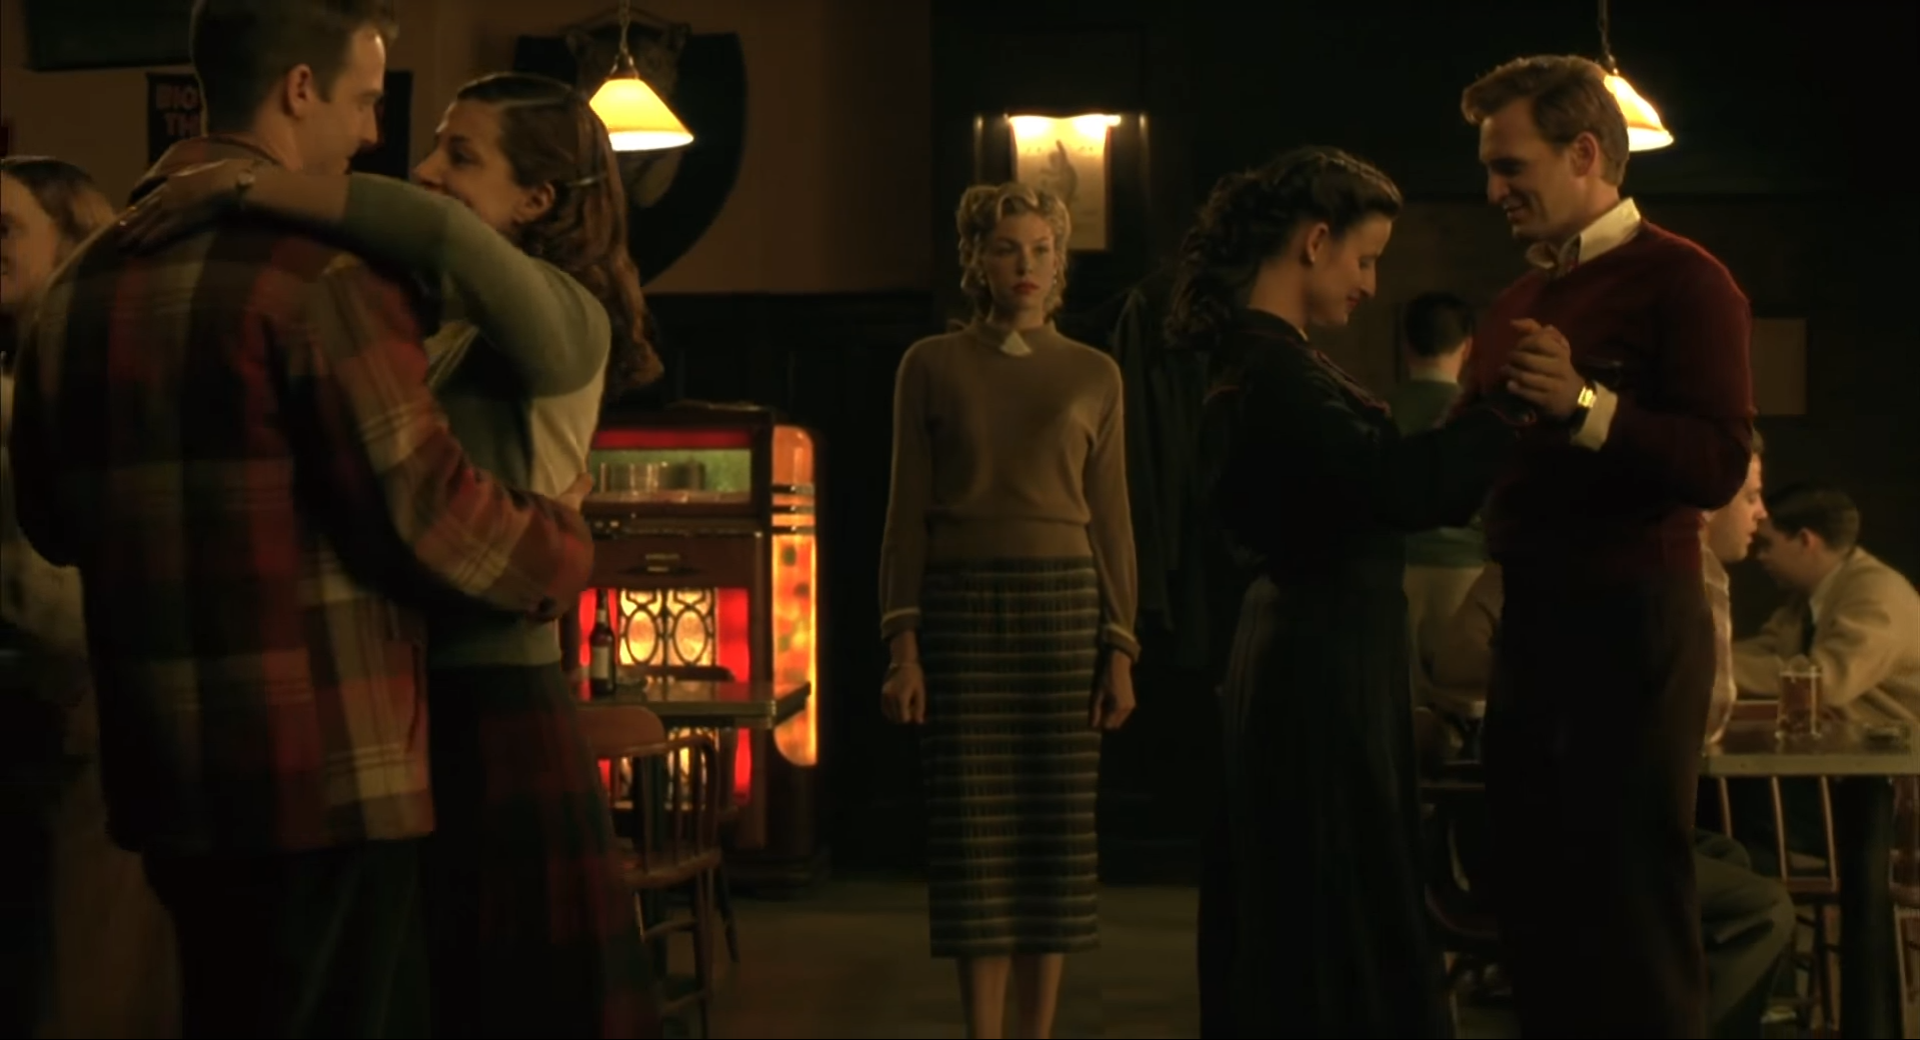
\includegraphics[width=1.0 \textwidth]{figures/blonde}
\end{frame}
\begin{frame}{PS2, Ex. 1: A Beautiful Mind}
  \begin{multicols}{2}
    As a "Game of Chicken":
    \begin{table}
      \begin{tabular}{cr|c|c|}
          & \multicolumn{1}{c}{} & \multicolumn{2}{c}{\color{blue}Hansen}\\
          \parbox[t]{1mm}{\multirow{3}{*}{\rotatebox[origin=c]{90}{\color{red}John Nash}}}
          & \multicolumn{1}{c}{} & \multicolumn{1}{c}{Brunette}  & \multicolumn{1}{c}{Blonde} \\\cline{3-4}
          & Brunette& 1, 1 & \textcolor{red}{1}, \textcolor{blue}{2}  \\\cline{3-4}
          & Blonde  & \textcolor{red}{2}, \textcolor{blue}{1} & 0, 0 \\\cline{3-4}
      \end{tabular}
    \end{table}
    Nash Equilibria (NE):
    $\{(Brunette,Blonde);(Blonde,Brunette)\}$
    Pareto Optimal (PO):\\
    $\{(Brunette,Blonde);(Blonde,Brunette)\}$
  \vfill\null \columnbreak
  \vfill\null
  \end{multicols}
\end{frame}
\begin{frame}{PS2, Ex. 1: A Beautiful Mind}
  \begin{multicols}{2}
    As a "Game of Chicken":
    \begin{table}
      \begin{tabular}{cr|c|c|}
          & \multicolumn{1}{c}{} & \multicolumn{2}{c}{\color{blue}Hansen}\\
          \parbox[t]{1mm}{\multirow{3}{*}{\rotatebox[origin=c]{90}{\color{red}John Nash}}}
          & \multicolumn{1}{c}{} & \multicolumn{1}{c}{Brunette}  & \multicolumn{1}{c}{Blonde} \\\cline{3-4}
          & Brunette& 1, 1 & \textcolor{red}{1}, \textcolor{blue}{2}  \\\cline{3-4}
          & Blonde  & \textcolor{red}{2}, \textcolor{blue}{1} & 0, 0 \\\cline{3-4}
      \end{tabular}
    \end{table}
    Nash Equilibria (NE):
    $\{(Brunette,Blonde);(Blonde,Brunette)\}$
    Pareto Optimal (PO):\\
    $\{(Brunette,Blonde);(Blonde,Brunette)\}$
  \vfill\null \columnbreak
    Can it be modelled to better reflect Hansen's view?
    \epigraph{"Nash, this is some way for you to get the blonde on your own... You can go to hell."}{\textit{- Hansen}}
  \vfill\null
  \end{multicols}
\end{frame}
\begin{frame}{PS2, Ex. 1: A Beautiful Mind}
Two ways of viewing the game depending on the degree of envy.
  \begin{multicols}{2}
    As a "Game of Chicken" (no envy):
    \begin{table}
      \begin{tabular}{cr|c|c|}
          & \multicolumn{1}{c}{} & \multicolumn{2}{c}{\color{blue}Hansen}\\
          \parbox[t]{1mm}{\multirow{3}{*}{\rotatebox[origin=c]{90}{\color{red}John Nash}}}
          & \multicolumn{1}{c}{} & \multicolumn{1}{c}{Brunette}  & \multicolumn{1}{c}{Blonde} \\\cline{3-4}
          & Brunette& 1, 1 & \textcolor{red}{1}, \textcolor{blue}{2}  \\\cline{3-4}
          & Blonde  & \textcolor{red}{2}, \textcolor{blue}{1} & 0, 0 \\\cline{3-4}
      \end{tabular}
    \end{table}
    Nash Equilibria (NE):
    $\{(Brunette,Blonde);(Blonde,Brunette)\}$
    Pareto Optimal (PO):\\
    $\{(Brunette,Blonde);(Blonde,Brunette)\}$
  \vfill\null \columnbreak
    As a "Prisoners' Dilemma" (high envy):
    \begin{table}
      \begin{tabular}{cr|c|c|}
          & \multicolumn{1}{c}{} & \multicolumn{2}{c}{\color{blue}Hansen}\\
          \parbox[t]{1mm}{\multirow{3}{*}{\rotatebox[origin=c]{90}{\color{red}John Nash}}}
          & \multicolumn{1}{c}{} & \multicolumn{1}{c}{Brunette}  & \multicolumn{1}{c}{Blonde} \\\cline{3-4}
          & Brunette& 1, 1 & -1, \textcolor{blue}{2}  \\\cline{3-4}
          & Blonde  & \textcolor{red}{2}, -1 & \textcolor{red}{0}, \textcolor{blue}{0} \\\cline{3-4}
      \end{tabular}
    \end{table}
    NE:\\
    $\{(Blonde,Blonde)\}$\\
    PO:\\
    Anything but $\{(Blonde,Blonde)\}$
  \vfill\null
  \end{multicols}
  \textbf{Def. Pareto Optimal:} No player can be better off without the other being worse off.
\end{frame}


\section{PS2, Ex. 2 (A): Nash Equilibria}

\begin{frame}{PS2, Ex. 2: Nash Equilibria}
  \begin{itemize}
    \item[a)] $NE=\{(T,L);(B,R)\}$
  \end{itemize}
  \begin{table}
    \begin{tabular}{c|c|c|}
        \multicolumn{1}{c}{} & \multicolumn{1}{c}{L}  & \multicolumn{1}{c}{R} \\\cline{2-3}
        T & \textcolor{blue}{9}, \textcolor{red}{9} & 0, 0 \\\cline{2-3}
        B & 0, 0 & \textcolor{blue}{8}, \textcolor{red}{8} \\\cline{2-3}
    \end{tabular}
  \end{table}
  \begin{itemize}
    \item[b)] $NE=\{(T,L);(B,R)\}$
  \end{itemize}
  \begin{table}
    \begin{tabular}{c|c|c|}
        \multicolumn{1}{c}{} & \multicolumn{1}{c}{L}  & \multicolumn{1}{c}{R} \\\cline{2-3}
        T & \textcolor{blue}{9}, \textcolor{red}{9} & 0, 7 \\\cline{2-3}
        B & 7, 0 & \textcolor{blue}{8}, \textcolor{red}{8} \\\cline{2-3}
    \end{tabular}
  \end{table}
  \begin{itemize}
    \item[c)] \textit{Which outcome is the most reasonable prediction in each game - and why?}
  \end{itemize}
\end{frame}
\begin{frame}{PS2, Ex. 2: Nash Equilibria}
  \begin{itemize}
    \item[a)] $NE=\{(T,L);(B,R)\}$
  \end{itemize}
  \begin{table}
    \begin{tabular}{c|c|c|}
        \multicolumn{1}{c}{} & \multicolumn{1}{c}{L}  & \multicolumn{1}{c}{R} \\\cline{2-3}
        T & \textcolor{blue}{9}, \textcolor{red}{9} & 0, 0 \\\cline{2-3}
        B & 0, 0 & \textcolor{blue}{8}, \textcolor{red}{8} \\\cline{2-3}
    \end{tabular}
  \end{table}
  \begin{itemize}
    \item[b)] $NE=\{(T,L);(B,R)\}$
  \end{itemize}
  \begin{table}
    \begin{tabular}{c|c|c|}
        \multicolumn{1}{c}{} & \multicolumn{1}{c}{L}  & \multicolumn{1}{c}{R} \\\cline{2-3}
        T & \textcolor{blue}{9}, \textcolor{red}{9} & 0, 7 \\\cline{2-3}
        B & 7, 0 & \textcolor{blue}{8}, \textcolor{red}{8} \\\cline{2-3}
    \end{tabular}
  \end{table}
  \begin{itemize}
    \item[c)] $\{T, L\}$ more reasonable as it's a pareto improvement of $\{B, R\}$.\\
    However, $\{B, R\}$ is more likely in b) if both players are risk averse.
  \end{itemize}
\end{frame}


\section{PS2, Ex. 3 (A): Elimination of weakly dominated strategies}

\begin{frame}{PS2, Ex. 3: Elimination of weakly dominated strategies}
  \begin{itemize}
    \item[a)] As opposed to IESDS, the order of elimination is crucial for iterated elimination of \textit{weakly} dominated pure strategies.
  \end{itemize}
  Example:
  \begin{table}
    \begin{tabular}{cc|c|c|}
        & \multicolumn{1}{c}{} & \multicolumn{2}{c}{Player 2}\\
        \parbox[t]{1mm}{\multirow{3}{*}{\rotatebox[origin=r]{90}{Player 1}}}
        & \multicolumn{1}{c}{} & \multicolumn{1}{c}{a}  & \multicolumn{1}{c}{b} \\\cline{3-4}
        & A & 0, 1 & 0, 0 \\\cline{3-4}
        & B & 0, 0 & 1, 0  \\\cline{3-4}
    \end{tabular}
  \end{table}
  \begin{itemize}
    \item[\nth{1} step:] Initially Player 1 can eliminate $A$ or Player 2 can eliminate $b$.
    \item[\nth{2} step:] In the reduced form game the other player can eliminate any strategy.
  \end{itemize}
\end{frame}
\begin{frame}{PS2, Ex. 3: Weak Domination}
  \begin{multicols}{2}
    \begin{itemize}
      \item[b)] $NE=\{(A,a);(B,a);(B,b)\}$
    \end{itemize}
    \begin{table}
      \begin{tabular}{cc|c|c|}
        & \multicolumn{1}{c}{} & \multicolumn{2}{c}{\color{blue}Player 2}\\
        \parbox[t]{1mm}{\multirow{3}{*}{\rotatebox[origin=r]{90}{\color{red}Player 1}}}
        & \multicolumn{1}{c}{} & \multicolumn{1}{c}{a}  & \multicolumn{1}{c}{b} \\\cline{3-4}
        & A & \textcolor{red}{0}, \textcolor{blue}{1} & 0, 0 \\\cline{3-4}
        & B & \textcolor{red}{0}, \textcolor{blue}{0} & \textcolor{red}{1}, \textcolor{blue}{0} \\\cline{3-4}
      \end{tabular}
    \end{table}
    $(B,a)$ is a NE as there is no incentive to deviate, i.e. either player is indifferent given the strategy of the other:
    \begin{align*}
        u_1(B,a)\geq u_1(A,a)\Leftrightarrow0\geq0\\
        u_2(B,a)\geq u_2(B,b)\Leftrightarrow0\geq0
    \end{align*}
    The (non-strict) inequalities can be turned around to explain the other equilibria:
    \begin{align*}
        u_1(B,a)\leq u_1(A,a)\Leftrightarrow0\leq0\\
        u_2(B,a)\leq u_2(B,b)\Leftrightarrow0\leq0
    \end{align*}
    \vfill\null \columnbreak
    \vfill\null
  \end{multicols}
\end{frame}
\begin{frame}{PS2, Ex. 3: Weak Domination}
  \begin{multicols}{2}
    \begin{itemize}
      \item[b)] $NE=\{(A,a);(B,a);(B,b)\}$
    \end{itemize}
    \begin{table}
      \begin{tabular}{cc|c|c|}
        & \multicolumn{1}{c}{} & \multicolumn{2}{c}{\color{blue}Player 2}\\
        \parbox[t]{1mm}{\multirow{3}{*}{\rotatebox[origin=r]{90}{\color{red}Player 1}}}
        & \multicolumn{1}{c}{} & \multicolumn{1}{c}{a}  & \multicolumn{1}{c}{b} \\\cline{3-4}
        & A & \textcolor{red}{0}, \textcolor{blue}{1} & 0, 0 \\\cline{3-4}
        & B & \textcolor{red}{0}, \textcolor{blue}{0} & \textcolor{red}{1}, \textcolor{blue}{0} \\\cline{3-4}
      \end{tabular}
    \end{table}
    $(B,a)$ is a NE as there is no incentive to deviate as either player is indifferent given the strategy of the other:
    \begin{align*}
        u_1(B,a)\geq u_1(A,a)\Leftrightarrow0\geq0\\
        u_2(B,a)\geq u_2(B,b)\Leftrightarrow0\geq0
    \end{align*}
    The (non-strict) inequalities can be turned around to explain the other equilibria:
    \begin{align*}
        u_1(B,a)\leq u_1(A,a)\Leftrightarrow0\leq0\\
        u_2(B,a)\leq u_2(B,b)\Leftrightarrow0\leq0
    \end{align*}
    \vfill\null \columnbreak
    As opposed to IESDS, iterated elimination of \textit{weakly} dominated pure strategies can eliminate NE. E.g. Player 1 can eliminate $A$ or Player 2 can eliminate $b$, eliminating one NE and giving us one of the reduced form games:
    \begin{table}
      \begin{subtable}{.5\columnwidth}
        \begin{tabular}{c|c|c|}
            \multicolumn{1}{c}{} & \multicolumn{1}{c}{a}  & \multicolumn{1}{c}{b} \\\cline{2-3}
            B & 0, 0 & 1, 0 \\\cline{2-3}
        \end{tabular}
      \end{subtable}% <---- don't forget this %
      \begin{subtable}{.5\columnwidth}
        \begin{tabular}{c|c|}
            \multicolumn{1}{c}{} & \multicolumn{1}{c}{a} \\\cline{2-2}
            A & 0, 1 \\\cline{2-2}
            B & 0, 0 \\\cline{2-2}
        \end{tabular}
      \end{subtable}
    \end{table}
    And another NE can be eliminated by further reducing to just one of the NE:
    \begin{table}
      \begin{subtable}{.33\columnwidth}
        \begin{tabular}{c|c|}
            \multicolumn{1}{c}{} & \multicolumn{1}{c}{a} \\\cline{2-2}
            B & 0, 0 \\\cline{2-2}
        \end{tabular}
      \end{subtable}% <---- don't forget this %
      \begin{subtable}{.33\columnwidth}
        \begin{tabular}{c|c|}
            \multicolumn{1}{c}{} & \multicolumn{1}{c}{b} \\\cline{2-2}
            B & 1, 0 \\\cline{2-2}
        \end{tabular}
      \end{subtable}% <---- don't forget this %
      \begin{subtable}{.33\columnwidth}
        \begin{tabular}{c|c|}
            \multicolumn{1}{c}{} & \multicolumn{1}{c}{a} \\\cline{2-2}
            A & 0, 1 \\\cline{2-2}
        \end{tabular}
      \end{subtable}
    \end{table}
  \vfill\null
\end{multicols}
\end{frame}


\section{PS2, Ex. 4-5: More Nash Equilibria}

\begin{frame}{PS2, Ex. 4-5: More Nash Equilibria}
  \begin{multicols}{2}
    \begin{itemize}
      \item[\textbf{4.}] Find all Nash equilibria in the following game:
    \end{itemize}
    \begin{table}
      \begin{tabular}{cc|c|c|c|}
          & \multicolumn{1}{c}{} & \multicolumn{3}{c}{Player 2}\\
          & \multicolumn{1}{c}{} & \multicolumn{1}{c}{a}  & \multicolumn{1}{c}{b} & \multicolumn{1}{c}{c} \\\cline{3-5}
          \parbox[t]{1mm}{\multirow{3}{*}{\rotatebox[origin=c]{90}{Player 1}}}
          & A & 7, 7 & 3, 0 & 1, 6 \\\cline{3-5}
          & B & 2, 8 & 5, 4 & 9, 3 \\\cline{3-5}
          & C & 3, 0 & 5, 4 & 2, 1 \\\cline{3-5}
      \end{tabular}
    \end{table}
  \vfill\null \columnbreak
    \begin{itemize}
      \item[\textbf{5.}] Find the Nash equilibrium in the following game:
    \end{itemize}
    \begin{table}
      \begin{tabular}{cc|c|c|}
          & \multicolumn{1}{c}{} & \multicolumn{2}{c}{Player 2}\\
          \parbox[t]{1mm}{\multirow{3}{*}{\rotatebox[origin=r]{90}{Player 1}}}
          & \multicolumn{1}{c}{} & \multicolumn{1}{c}{A}  & \multicolumn{1}{c}{B} \\\cline{3-4}
          & A & 100, 100 & 1, 99 \\\cline{3-4}
          & B & 99, 1 & 0, 0 \\\cline{3-4}
      \end{tabular}
    \end{table}
    Find the NE after adding 2 to the payoff of strategy B for each player:
    \begin{table}
      \begin{tabular}{cc|c|c|}
          & \multicolumn{1}{c}{} & \multicolumn{2}{c}{Player 2}\\
          \parbox[t]{1mm}{\multirow{3}{*}{\rotatebox[origin=r]{90}{Player 1}}}
          & \multicolumn{1}{c}{} & \multicolumn{1}{c}{A}  & \multicolumn{1}{c}{B} \\\cline{3-4}
          & A & 100, 100 & 1, 101 \\\cline{3-4}
          & B & 101, 1 & 2, 2 \\\cline{3-4}
      \end{tabular}
    \end{table}
    \textit{Comment. What has changed?}
  \vfill\null
  \end{multicols}
\end{frame}
\begin{frame}{PS2, Ex. 4-5: More Nash Equilibria}
  \begin{multicols}{2}
    \begin{itemize}
      \item[\textbf{4.}] Find all Nash equilibria in the following game:
    \end{itemize}
    \begin{table}
      \begin{tabular}{cc|c|c|c|}
          & \multicolumn{1}{c}{} & \multicolumn{3}{c}{\color{blue}Player 2}\\
          & \multicolumn{1}{c}{} & \multicolumn{1}{c}{a}  & \multicolumn{1}{c}{b} & \multicolumn{1}{c}{c} \\\cline{3-5}
          \parbox[t]{1mm}{\multirow{3}{*}{\rotatebox[origin=c]{90}{\color{red}Player 1}}}
          & A & \textcolor{red}{7}, \textcolor{blue}{7} & 3, 0 & 1, 6 \\\cline{3-5}
          & B & 2, \textcolor{blue}{8} & \textcolor{red}{5}, 4 & \textcolor{red}{9}, 3 \\\cline{3-5}
          & C & 3, 0 & \textcolor{red}{5}, \textcolor{blue}{4} & 2, 1 \\\cline{3-5}
      \end{tabular}
    \end{table}
    $NE=\{(A,a);(C,b)\}$ as there is no incentive to deviate for any player, e.g.
    \begin{align*}
        u_1(C,b)\geq u_1(B,b)\Leftrightarrow5\geq5
    \end{align*}
    Player $1$ is indifferent between $(A,b)$ and $(B,b)$, but Player $1$ knows that Player $2$'s best response to $B$ would be $a$.
  \vfill\null \columnbreak
    \begin{itemize}
      \item[\textbf{5.}] Find the Nash equilibrium in the following game:
    \end{itemize}
    \begin{table}
      \begin{tabular}{cc|c|c|}
          & \multicolumn{1}{c}{} & \multicolumn{2}{c}{Player 2}\\
          \parbox[t]{1mm}{\multirow{3}{*}{\rotatebox[origin=r]{90}{Player 1}}}
          & \multicolumn{1}{c}{} & \multicolumn{1}{c}{A}  & \multicolumn{1}{c}{B} \\\cline{3-4}
          & A & 100, 100 & 1, 99 \\\cline{3-4}
          & B & 99, 1 & 0, 0 \\\cline{3-4}
      \end{tabular}
    \end{table}
    Find the NE after adding 2 to the payoff of strategy B for each player:
    \begin{table}
      \begin{tabular}{cc|c|c|}
          & \multicolumn{1}{c}{} & \multicolumn{2}{c}{Player 2}\\
          \parbox[t]{1mm}{\multirow{3}{*}{\rotatebox[origin=r]{90}{Player 1}}}
          & \multicolumn{1}{c}{} & \multicolumn{1}{c}{A}  & \multicolumn{1}{c}{B} \\\cline{3-4}
          & A & 100, 100 & 1, 101 \\\cline{3-4}
          & B & 101, 1 & 2, 2 \\\cline{3-4}
      \end{tabular}
    \end{table}
    \textit{Comment. What has changed?}
  \vfill\null
  \end{multicols}
\end{frame}
\begin{frame}{PS2, Ex. 4-5: More Nash Equilibria}
  \begin{multicols}{2}
    \begin{itemize}
      \item[\textbf{4.}] Find all Nash equilibria in the following game:
    \end{itemize}
    \begin{table}
      \begin{tabular}{cc|c|c|c|}
          & \multicolumn{1}{c}{} & \multicolumn{3}{c}{\color{blue}Player 2}\\
          & \multicolumn{1}{c}{} & \multicolumn{1}{c}{a}  & \multicolumn{1}{c}{b} & \multicolumn{1}{c}{c} \\\cline{3-5}
          \parbox[t]{1mm}{\multirow{3}{*}{\rotatebox[origin=c]{90}{\color{red}Player 1}}}
          & A & \textcolor{red}{7}, \textcolor{blue}{7} & 3, 0 & 1, 6 \\\cline{3-5}
          & B & 2, \textcolor{blue}{8} & \textcolor{red}{5}, 4 & \textcolor{red}{9}, 3 \\\cline{3-5}
          & C & 3, 0 & \textcolor{red}{5}, \textcolor{blue}{4} & 2, 1 \\\cline{3-5}
      \end{tabular}
    \end{table}
    $NE=\{(A,a);(C,b)\}$ as there is no incentive to deviate for any player, e.g.
    \begin{align*}
        u_1(C,b)\geq u_1(B,b)\Leftrightarrow5\geq5
    \end{align*}
    Player $1$ is indifferent between $(A,b)$ and $(B,b)$, but Player $1$ knows that Player $2$'s best response to $B$ would be $a$.
  \vfill\null \columnbreak
    \begin{itemize}
      \item[\textbf{5.}] Find the Nash equilibrium in the following game:
    \end{itemize}
    \begin{table}
      \begin{tabular}{cc|c|c|}
          & \multicolumn{1}{c}{} & \multicolumn{2}{c}{\color{blue}Player 2}\\
          \parbox[t]{1mm}{\multirow{3}{*}{\rotatebox[origin=r]{90}{\color{red}Player 1}}}
          & \multicolumn{1}{c}{} & \multicolumn{1}{c}{\textcolor{blue}{A}}  & \multicolumn{1}{c}{B} \\\cline{3-4}
          & \textcolor{red}{A} & \textcolor{red}{100}, \textcolor{blue}{100} & \textcolor{red}{1}, 99 \\\cline{3-4}
          & B & 99, \textcolor{blue}{1} & 0, 0 \\\cline{3-4}
      \end{tabular}
    \end{table}
    Find the NE after adding 2 to the payoff of strategy B for each player:
    \begin{table}
      \begin{tabular}{cc|c|c|}
          & \multicolumn{1}{c}{} & \multicolumn{2}{c}{Player 2}\\
          \parbox[t]{1mm}{\multirow{3}{*}{\rotatebox[origin=r]{90}{Player 1}}}
          & \multicolumn{1}{c}{} & \multicolumn{1}{c}{A}  & \multicolumn{1}{c}{B} \\\cline{3-4}
          & A & 100, 100 & 1, 101 \\\cline{3-4}
          & B & 101, 1 & 2, 2 \\\cline{3-4}
      \end{tabular}
    \end{table}
    \textit{Comment. What has changed?}
  \vfill\null
  \end{multicols}
\end{frame}
\begin{frame}{PS2, Ex. 4-5: More Nash Equilibria}
  \begin{multicols}{2}
    \begin{itemize}
      \item[\textbf{4.}] Find all Nash equilibria in the following game:
    \end{itemize}
    \begin{table}
      \begin{tabular}{cc|c|c|c|}
          & \multicolumn{1}{c}{} & \multicolumn{3}{c}{\color{blue}Player 2}\\
          & \multicolumn{1}{c}{} & \multicolumn{1}{c}{a}  & \multicolumn{1}{c}{b} & \multicolumn{1}{c}{c} \\\cline{3-5}
          \parbox[t]{1mm}{\multirow{3}{*}{\rotatebox[origin=c]{90}{\color{red}Player 1}}}
          & A & \textcolor{red}{7}, \textcolor{blue}{7} & 3, 0 & 1, 6 \\\cline{3-5}
          & B & 2, \textcolor{blue}{8} & \textcolor{red}{5}, 4 & \textcolor{red}{9}, 3 \\\cline{3-5}
          & C & 3, 0 & \textcolor{red}{5}, \textcolor{blue}{4} & 2, 1 \\\cline{3-5}
      \end{tabular}
    \end{table}
    $NE=\{(A,a);(C,b)\}$ as there is no incentive to deviate for any player, e.g.
    \begin{align*}
        u_1(C,b)\geq u_1(B,b)\Leftrightarrow5\geq5
    \end{align*}
    Player $1$ is indifferent between $(A,b)$ and $(B,b)$, but Player $1$ knows that Player $2$'s best response to $B$ would be $a$.
  \vfill\null \columnbreak
    \begin{itemize}
      \item[\textbf{5.}] Find the Nash equilibrium in the following game:
    \end{itemize}
    \begin{table}
      \begin{tabular}{cc|c|c|}
          & \multicolumn{1}{c}{} & \multicolumn{2}{c}{\color{blue}Player 2}\\
          \parbox[t]{1mm}{\multirow{3}{*}{\rotatebox[origin=r]{90}{\color{red}Player 1}}}
          & \multicolumn{1}{c}{} & \multicolumn{1}{c}{\textcolor{blue}{A}}  & \multicolumn{1}{c}{\sout{B}} \\\cline{3-4}
          & \textcolor{red}{A} & \textcolor{red}{100}, \textcolor{blue}{100} & \sout{\textcolor{red}{1}, 99} \\\cline{3-4}
          & \sout{B} & \sout{99, \textcolor{blue}{1}} & \sout{0, 0} \\\cline{3-4}
      \end{tabular}
    \end{table}
    Find the NE after adding 2 to the payoff of strategy B for each player:
    \begin{table}
      \begin{tabular}{cc|c|c|}
          & \multicolumn{1}{c}{} & \multicolumn{2}{c}{\color{blue}Player 2}\\
          \parbox[t]{1mm}{\multirow{3}{*}{\rotatebox[origin=r]{90}{\color{red}Player 1}}}
          & \multicolumn{1}{c}{} & \multicolumn{1}{c}{A}  & \multicolumn{1}{c}{\textcolor{blue}{B}} \\\cline{3-4}
          & A & 100, 100 & 1, \textcolor{blue}{101} \\\cline{3-4}
          & \textcolor{red}{B} & \textcolor{red}{101}, 1 & \textcolor{red}{2}, \textcolor{blue}{2} \\\cline{3-4}
      \end{tabular}
    \end{table}
    \textit{Comment. What has changed?}
  \vfill\null
  \end{multicols}
\end{frame}
\begin{frame}{PS2, Ex. 4-5: More Nash Equilibria}
  \begin{multicols}{2}
    \begin{itemize}
      \item[\textbf{4.}] Find all Nash equilibria in the following game:
    \end{itemize}
    \begin{table}
      \begin{tabular}{cc|c|c|c|}
          & \multicolumn{1}{c}{} & \multicolumn{3}{c}{\color{blue}Player 2}\\
          & \multicolumn{1}{c}{} & \multicolumn{1}{c}{a}  & \multicolumn{1}{c}{b} & \multicolumn{1}{c}{c} \\\cline{3-5}
          \parbox[t]{1mm}{\multirow{3}{*}{\rotatebox[origin=c]{90}{\color{red}Player 1}}}
          & A & \textcolor{red}{7}, \textcolor{blue}{7} & 3, 0 & 1, 6 \\\cline{3-5}
          & B & 2, \textcolor{blue}{8} & \textcolor{red}{5}, 4 & \textcolor{red}{9}, 3 \\\cline{3-5}
          & C & 3, 0 & \textcolor{red}{5}, \textcolor{blue}{4} & 2, 1 \\\cline{3-5}
      \end{tabular}
    \end{table}
    $NE=\{(A,a);(C,b)\}$ as there is no incentive to deviate for any player, e.g.
    \begin{align*}
        u_1(C,b)\geq u_1(B,b)\Leftrightarrow5\geq5
    \end{align*}
    Player $1$ is indifferent between $(A,b)$ and $(B,b)$, but Player $1$ knows that Player $2$'s best response to $B$ would be $a$.
  \vfill\null \columnbreak
    \begin{itemize}
      \item[\textbf{5.}] Find the Nash equilibrium in the following game:
    \end{itemize}
    \begin{table}
      \begin{tabular}{cc|c|c|}
          & \multicolumn{1}{c}{} & \multicolumn{2}{c}{\color{blue}Player 2}\\
          \parbox[t]{1mm}{\multirow{3}{*}{\rotatebox[origin=r]{90}{\color{red}Player 1}}}
          & \multicolumn{1}{c}{} & \multicolumn{1}{c}{\textcolor{blue}{A}}  & \multicolumn{1}{c}{\sout{B}} \\\cline{3-4}
          & \textcolor{red}{A} & \textcolor{red}{100}, \textcolor{blue}{100} & \sout{\textcolor{red}{1}, 99} \\\cline{3-4}
          & \sout{B} & \sout{99, \textcolor{blue}{1}} & \sout{0, 0} \\\cline{3-4}
      \end{tabular}
    \end{table}
    Find the NE after adding 2 to the payoff of strategy B for each player:
    \begin{table}
      \begin{tabular}{cc|c|c|}
          & \multicolumn{1}{c}{} & \multicolumn{2}{c}{\color{blue}Player 2}\\
          \parbox[t]{1mm}{\multirow{3}{*}{\rotatebox[origin=r]{90}{\color{red}Player 1}}}
          & \multicolumn{1}{c}{} & \multicolumn{1}{c}{\sout{A}}  & \multicolumn{1}{c}{\textcolor{blue}{B}} \\\cline{3-4}
          & \sout{A} & \sout{100, 100} & \sout{1, \textcolor{blue}{101}} \\\cline{3-4}
          & \textcolor{red}{B} & \sout{\textcolor{red}{101}, 1} & \textcolor{red}{2}, \textcolor{blue}{2} \\\cline{3-4}
      \end{tabular}
    \end{table}
    Now B is strictly dominated by A instead.\\
    $NE = \{B, B\}$ as coordination on $\{A, A\}$ isn't credible due to incentive to deviates.
  \vfill\null
  \end{multicols}
\end{frame}


\section{PS2, Ex. 6: Cournot equilibrium}

\begin{frame}{PS2, Ex. 6: Cournot equilibrium}
  \begin{multicols}{2}
    There are two bakeries in the same village. Every morning, they simultaneously decide how many breads to produce. Denote the quantities they produce by $q_1$ and $q_2$. The price for which they can sell the bread is a function of the overall quantity, such that $p=11-(q_1+q_2)$. The cost of producing one bread is $2$.
    \begin{itemize}
      \item[a)] Compute the quantities in the Cournot equilibrium, i.e., the Nash Equilibrium of the game where the firms simultaneously choose quantities.
      \item[b)]  Draw a diagram of the best response functions, and check whether they really intersect in the Nash Equilibrium.
    \end{itemize}
  \vfill\null \columnbreak
   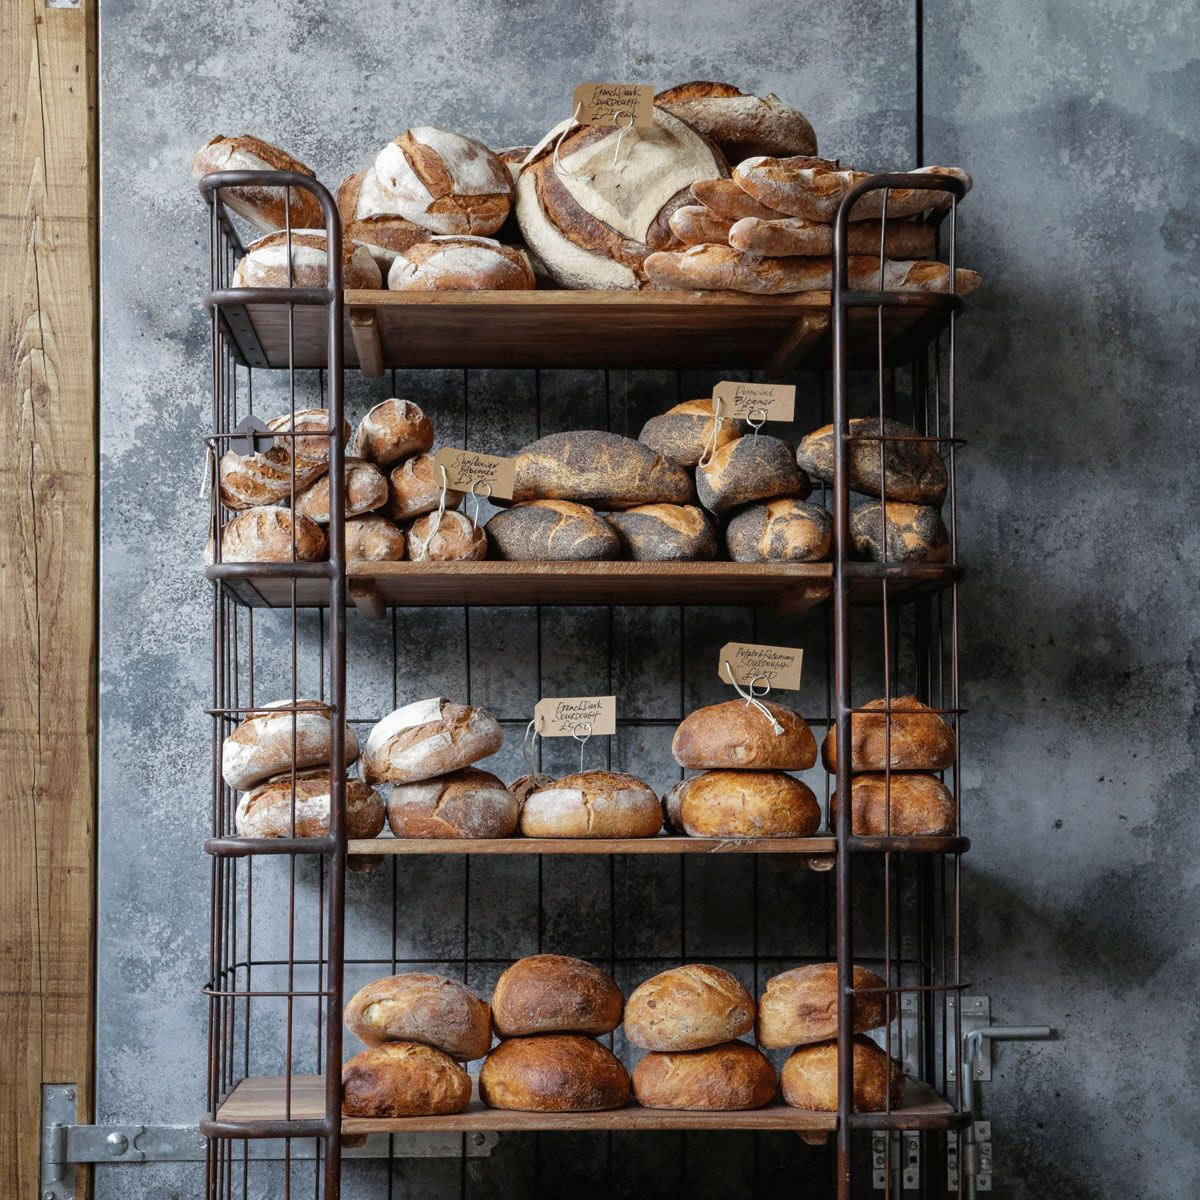
\includegraphics[width=.5 \textwidth]{figures/bread}
  \vfill\null
  \end{multicols}
\end{frame}
\begin{frame}{PS2, Ex. 6: Cournot equilibrium}
  \begin{multicols}{2}
    There are two bakeries in the same village. Every morning, they simultaneously decide how many breads to produce. Denote the quantities they produce by $q_1$ and $q_2$. The price for which they can sell the bread is a function of the overall quantity, such that $p=11-(q_1+q_2)$. The cost of producing one bread is $2$.
    \begin{itemize}
      \item[a)] Compute the quantities in the Cournot equilibrium, i.e., the Nash Equilibrium of the game where the firms simultaneously choose quantities.
      \item[b)]  Draw a diagram of the best response functions, and check whether they really intersect in the Nash Equilibrium.
    \end{itemize}
  \vfill\null \columnbreak
    Cookbook (general, not just for bread):
    \begin{enumerate}
      \item Write up the payoff (profit) functions and take the derivative with respect to one's quantity.
      \item From the first order conditions (FOCs) find the Best-Response (BR) functions given the quantity chosen by the other player.
      \item Substitute in the BR quantity for the other player to solve for the equilibrium quantities.
    \end{enumerate}
  \vfill\null
  \end{multicols}
\end{frame}
\begin{frame}{PS2, Ex. 6: Cournot equilibrium}
  \begin{multicols}{2}
    \begin{itemize}
      \item[a)] Quantities in the Cournot equilibrium
    \end{itemize}
    Inverse market demand is given as:
    \begin{align}
      p = 11 - (q_1+q_2) \label{p}
    \end{align}
    The payoff (profit) for firm $i$ with constant marginal cost $c=2$ is:
    \begin{align}
        \pi_i&=(p-c)q_i \nonumber\\
             &=(11-q_i-q_j-2)q_i\nonumber\\
             &=(9-q_i-q_j)q_i\text{ for }i\in\{1,2\}
      \label{payoff}
    \end{align}
    FOC of the payoff function \eqref{payoff} for firm $i$:
    \begin{align}
        \frac{\delta\pi_i}{\delta q_i}=9-2q_i-q_j&=0\nonumber\\
        \Rightarrow q_i &= \frac{9-q_j}{2}
      \label{br}
    \end{align}
    This is firm $i$'s Best-Response (BR) function given the quantity chosen by the other firm $j$.
  \vfill\null \columnbreak
    Due to the symmetry of the payoff functions the Best-Response quantity $q_i^{*}=q_j^{*}$ which we insert in \eqref{br} to find the equilibrium quantities:
    \begin{align}
        q_i^{*} &= \frac{9-q_i^{*}}{2}\nonumber\\
        \frac{3}{2}q_i^{*} &= \frac{9}{2}\nonumber\\
        q_i^{*} &= \frac{2}{3}\cdot\frac{9}{2}\nonumber\\
        q_i^{*} &= 3
        \label{ne}
    \end{align}
    I.e. the Cournot/Nash equilibrium is:
    \begin{align*}
      q_i^{*}=q_j^{*}=3\equiv q^{NE}
    \end{align*}
  \vfill\null
  \end{multicols}
\end{frame}
\begin{frame}{PS2, Ex. 6: Cournot equilibrium}
    \begin{itemize}
      \item[b)] To plot the intersection we need:
      \begin{itemize}\normalsize
        \item The inverse of the BR function for firm 1: $q_1(q_2) = \frac{9-q_2}{2} \Rightarrow q_2 = 9-2q_1$
        \item And the BR function for firm 2: $q_2 = \frac{9-q_1}{2}$
      \end{itemize}
    \end{itemize}
   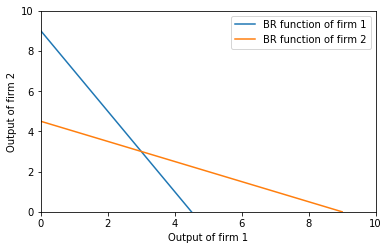
\includegraphics[width=1 \textwidth]{figures/br}
\end{frame}


\section{PS2, Ex. 7: Letter from an American foundation}

\begin{frame}{PS2, Ex. 7: Letter from an American foundation}
  \begin{multicols}{2}
    Heidi and Jakup have both received a letter from an American foundation:\\\medskip
    We are willing to give the two of you one million US dollars in total. There are, however, some conditions involved. Take a pen and a paper, write down how much you would like to get and send it to us in a sealed envelope. If the sum of your two claims is equal to or below one million, you get exactly what you have asked for. Otherwise you get punished for being greedy - none of you gets a single cent.\\\medskip
    Unfortunately, they do not know how to get hold of each other before answering, so there is no chance for them to communicate before sending the envelope.
  \vfill\null \columnbreak
    \begin{itemize}
      \item[a)] What would you write, if you were one of them?
      \item[b)] Formalize the game. Find all the pure-strategy Nash equilibria.
      \item[c)] What do you think, which of the equilibria is much more likely to be played in reality? Does it correspond to your answer to a)?
      \item[d)] If they had time to communicate with each other, what do you think would happen? What would you do, if you were one of them?
      \item[e)] Now assume that Heidi could send a message to Jakup, but Jakup would not be able to answer. What advice would you give to Heidi?
    \end{itemize}
  \vfill\null
  \end{multicols}
\end{frame}
\begin{frame}{PS2, Ex. 7: Letter from an American foundation}
  \begin{multicols}{2}
    \begin{itemize}
      \item[b)] The normal form game:
    \end{itemize}
    Players: \begin{align*}I={Heidi,Jakup}\end{align*}
    Strategy set: \begin{align*}
      S_i = \{0; 0.01; ... ; 99999.99; 1000000\}\end{align*}
    Payoffs for player $i\neq j$: \begin{align*}
      u_i(s_i,s_j)=
      \left\{ \begin{array}{ccl}
      s_i & \mbox{if} & s_i+s_j \leq 1000000 \\
      0   & \mbox{if} & s_i+s_j > 1000000
      \end{array}\right. \end{align*}
    Pure Strategy Nash Equilibria (PSNE): \begin{align*} \{(s_1; s_2)\in S_1\times S_2 : s_1 + s_2 = 1000000\} \end{align*}
  \vfill\null \columnbreak
    \begin{itemize}
      \item[c)] What do you think, which of the equilibria is much more likely to be played in reality? Does it correspond to your answer to a)?
      \item[d)] If they had time to communicate with each other, what do you think would happen? What would you do, if you were one of them?
      \item[e)] Now assume that Heidi could send a message to Jakup, but Jakup would not be able to answer. What advice would you give to Heidi?
    \end{itemize}
  \vfill\null
  \end{multicols}
\end{frame}
\begin{frame}{PS2, Ex. 7: Letter from an American foundation}
  \begin{multicols}{2}
    \begin{itemize}
      \item[b)] The normal form game:
    \end{itemize}
    Players: \begin{align*}I={Heidi,Jakup}\end{align*}
    Strategy set: \begin{align*}
      S_i = \{0; 0.01; ... ; 99999.99; 1000000\}\end{align*}
    Payoffs for player $i\neq j$: \begin{align*}
      u_i(s_i,s_j)=
      \left\{ \begin{array}{ccl}
      s_i & \mbox{if} & s_i+s_j \leq 1000000 \\
      0   & \mbox{if} & s_i+s_j > 1000000
      \end{array}\right. \end{align*}
    Pure Strategy Nash Equilibria (PSNE): \begin{align*} \{(s_1; s_2)\in S_1\times S_2 : s_1 + s_2 = 1000000\} \end{align*}
  \vfill\null \columnbreak
    \begin{itemize}
      \item[e)] Now assume that Heidi could send a message to Jakup, but Jakup would not be able to answer. What advice would you give to Heidi?
    \end{itemize}
    Heidi can either play it safe by sending the message that she will write 500000.\\\medskip
    Or try to pressure Jakup to accept an unequal equilibrium, e.g. send the message "I will write 800000, you can write 200000 or get nothing."
  \vfill\null
  \end{multicols}
\end{frame}


\section{PS2, Ex. 8: Stopping the bike thief}

\begin{frame}{PS2, Ex. 8: Stopping the bike thief}
  \begin{multicols}{2}
    There are $n$ people observing someone trying to steal a parked bike. Each of the witnesses would like the thief to be stopped, but prefers not to do it him/herself (because it is unpleasant and perhaps even dangerous). More precisely, if the thief is stopped by someone else, each of the witnesses gets a utility of $v > 0$. Every person who stops the thief gets a utility of $v-c>0$, where $c$ is the cost of interaction with the thief. Finally, if nobody stops the thief and the bike gets stolen, every witness gets a utility of $0$. The witnesses decide whether or not to stop the thief simultaneously and independently.
  \vfill\null \columnbreak
    \begin{itemize}
      \item[a)] Write the game in normal form.
      \item[b)] Describe all pure-strategy Nash equilibria of the game (an informal description is sufficient). It may be a good idea to start with the case $n = 2$.
    \end{itemize}
    
\includegraphics[width=.5 \textwidth]{figures/bike_thief}
  \vfill\null
  \end{multicols}
\end{frame}
\begin{frame}{PS2, Ex. 8: Stopping the bike thief}
    \begin{itemize}
      \item[a)] Write the game in normal form:
    \end{itemize}
    Players: $I={1, 2, ..., n}$\\
    Strategy set: $S_i = \{\text{Do nothing}; \text{Stop the thief}\}$\\
    Payoffs for player $i\neq j$: \begin{align*}
      u_i(s_i,s_j)=
      \left\{ \begin{array}{rl}
      v > 0 & \mbox{if I do nothing and someone else stops the thief} \\
      v-c>0 & \mbox{if I stop the thief} \\
      0     & \mbox{if nobody stops the thief}
      \end{array}\right. \end{align*}
    \begin{itemize}
      \item[b)] Describe all pure-strategy Nash equilibria of the game (an informal description is sufficient). It may be a good idea to start with the case $n = 2$.
    \end{itemize}
\end{frame}
\begin{frame}{PS2, Ex. 8: Stopping the bike thief}
    \begin{itemize}
      \item[a)] Write the game in normal form:
    \end{itemize}
    Players: $I={1, 2, ..., n}$\\
    Strategy set: $S_i = \{\text{\text{Stop the thief}; Do nothing}\}$\\
    Payoffs for player $i\neq j$: \begin{align*}
      u_i(s_i,s_j)=
      \left\{ \begin{array}{rl}
      v > 0 & \mbox{if I do nothing and someone else stops the thief} \\
      v-c>0 & \mbox{if I stop the thief} \\
      0     & \mbox{if nobody stops the thief}
      \end{array}\right. \end{align*}
    \begin{itemize}
      \item[b)] Describe all pure-strategy Nash equilibria of the game (an informal description is sufficient). It may be a good idea to start with the case $n = 2$.
    \end{itemize}
    If $c>0$, there exist $n$ equilibria where exactly one person stops the thief, e.g.:
    \begin{table}
      \begin{tabular}{cc|c|c|}
        & \multicolumn{1}{c}{} & \multicolumn{2}{c}{\color{blue}Player 2}\\
        \parbox[t]{1mm}{\multirow{3}{*}{\rotatebox[origin=r]{90}{\color{red}Player 1}}}
        & \multicolumn{1}{c}{} & \multicolumn{1}{c}{Stop the thief}  & \multicolumn{1}{c}{Do nothing} \\\cline{3-4}
        & Stop the thief & $v-c$ ; $v-c$ & \textcolor{red}{$v-c$} ; \textcolor{blue}{$v$} \\\cline{3-4}
        & Do nothing & \textcolor{red}{$v$} ; \textcolor{blue}{$v-c$} & 0 ; 0 \\\cline{3-4}
      \end{tabular}
    \end{table}
\end{frame}



% \section{PS2, Ex. }
%
% \begin{frame}{PS2, Ex. }
%   \begin{multicols}{2}
%     \begin{table}
%       \begin{tabular}{cc|c|c|}
%           & \multicolumn{1}{c}{} & \multicolumn{2}{c}{Player 2}\\
%           \parbox[t]{1mm}{\multirow{3}{*}{\rotatebox[origin=r]{90}{Player 1}}}
%           & \multicolumn{1}{c}{} & \multicolumn{1}{c}{A}  & \multicolumn{1}{c}{B} \\\cline{3-4}
%           & A &  &  \\\cline{3-4}
%           & B &  &  \\\cline{3-4}
%       \end{tabular}
%     \end{table}
%   \vfill\null \columnbreak
%     \begin{table}
%       \begin{tabular}{cc|c|c|}
%         & \multicolumn{1}{c}{} & \multicolumn{2}{c}{\color{blue}Player 2}\\
%         \parbox[t]{1mm}{\multirow{3}{*}{\rotatebox[origin=r]{90}{\color{red}Player 1}}}
%         & \multicolumn{1}{c}{} & \multicolumn{1}{c}{A}  & \multicolumn{1}{c}{B} \\\cline{3-4}
%         & A & \textcolor{red}{}, \textcolor{blue}{} &   \\\cline{3-4}
%         & B &  &  \\\cline{3-4}
%       \end{tabular}
%     \end{table}
%     \begin{table}
%       \begin{tabular}{c|c|c|}
%           \multicolumn{1}{c}{} & \multicolumn{1}{c}{A}  & \multicolumn{1}{c}{B} \\\cline{2-3}
%           A &  &  \\\cline{2-3}
%           B &  &  \\\cline{2-3}
%       \end{tabular}
%     \end{table}
%   \vfill\null
%   \end{multicols}
% \end{frame}



% \begin{frame}%{References}
%   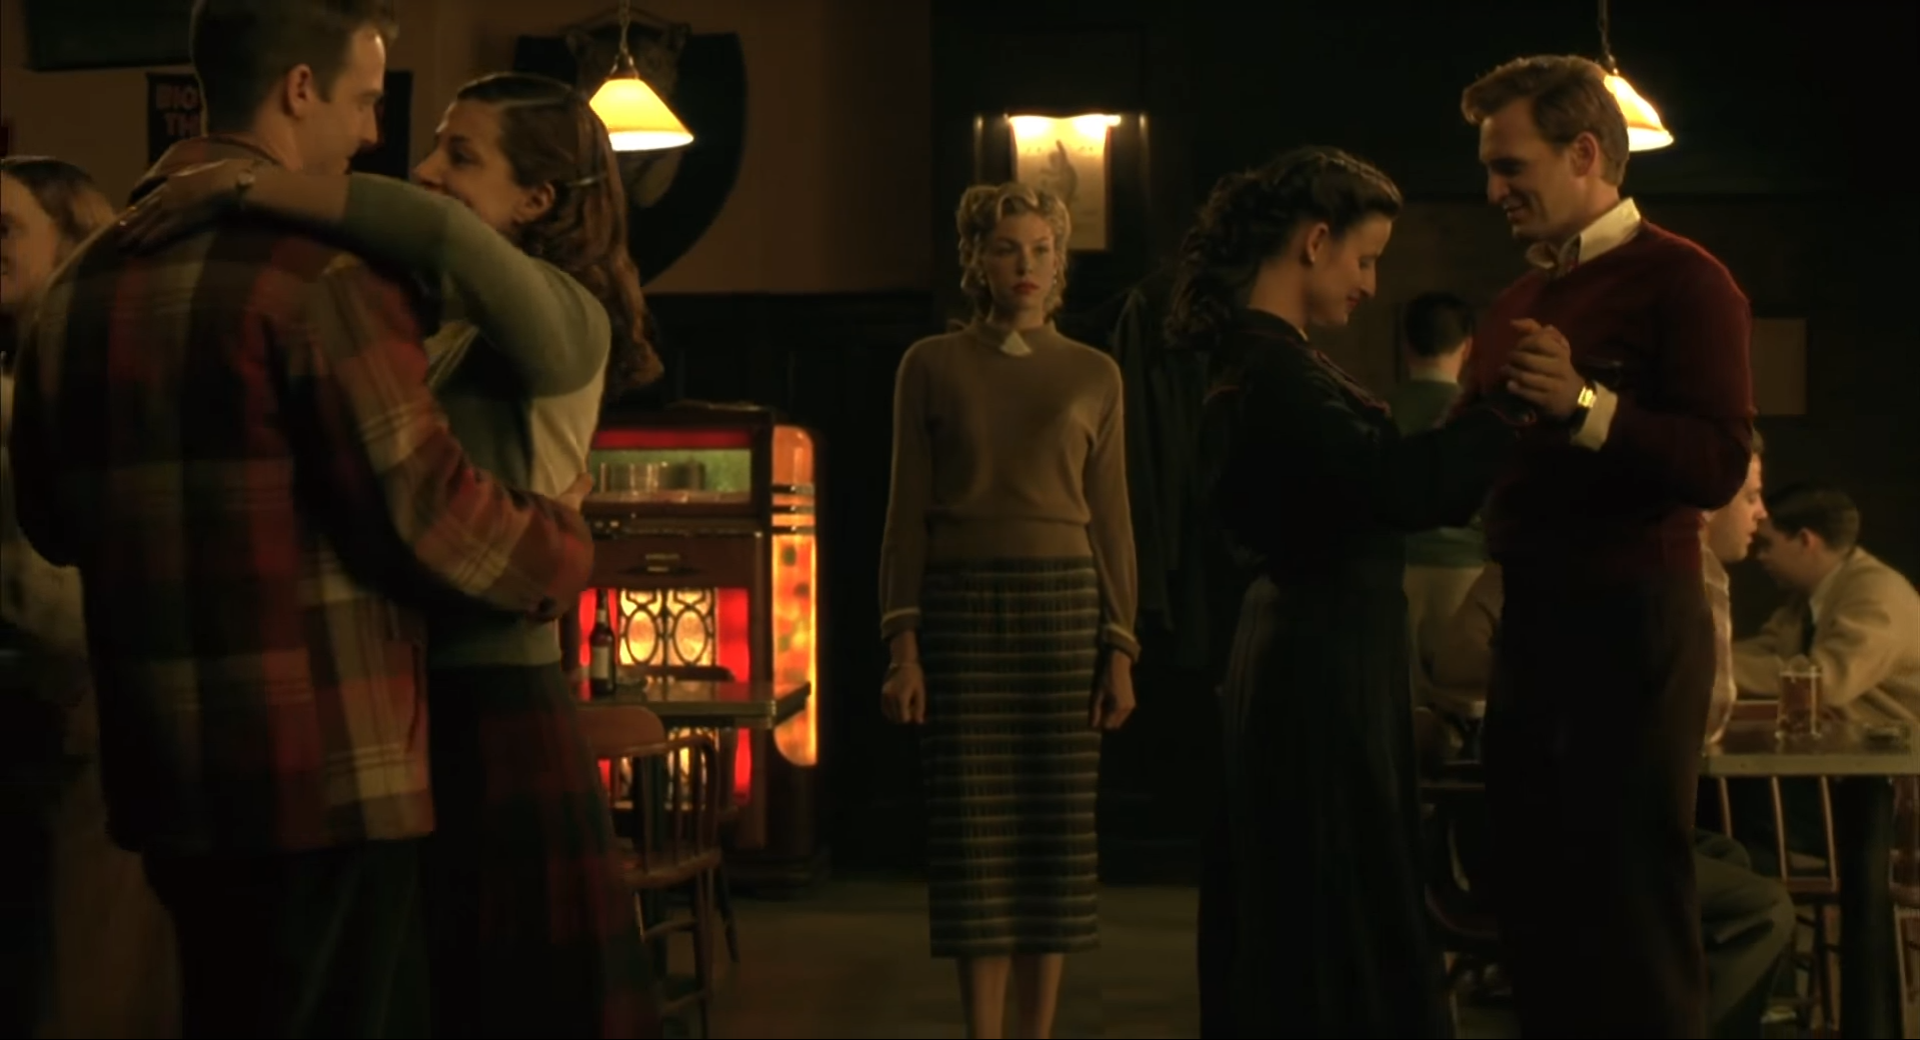
\includegraphics[width=1.0 \textwidth]{figures/blonde}
%   \printbibliography
% \end{frame}

\end{document}
